\documentclass[12pt]{article}

\usepackage[hmargin=1in,vmargin=1in]{geometry}
\usepackage{parskip}
\usepackage{hyperref}
\usepackage{graphicx}
\usepackage{color}
\usepackage{verbatim}
\hypersetup{pdfstartview=FitV,hidelinks}



\begin{document}

{
  \Large
  \centering
  {\bf Lab 10 -- Estimating abundance with
    capture-mark-recapture data} \\
  Due before your next lab \par
}

\vspace{10pt}

% Analysis of the (fake) Mongolian gazelle ({\it Procapra gutturosa})
% data using program DISTANCE.

The purpose of this lab is to learn how to %use program MARK to
estimate abundance using mark-recapture data. You will also learn how
to use program MARK. Put your answers in a Word file and upload it to
ELC. Name the file something like ``Chandler-lab10.docx''. Due before
your next lab.




%\clearpage

\section*{\large Part I: Lincoln-Peterson estimation}
Suppose you capture, mark, and release 100 largmouth bass at Lake
Herrick. The next day, you return and capture 50 individuals, 25 of
which were marked on the first occasion. What is the Lincoln-Peterson
estimate of abundance ($N$)? Show your work.

% \begin{figure}[h!]
%   \centering
%   \fbox{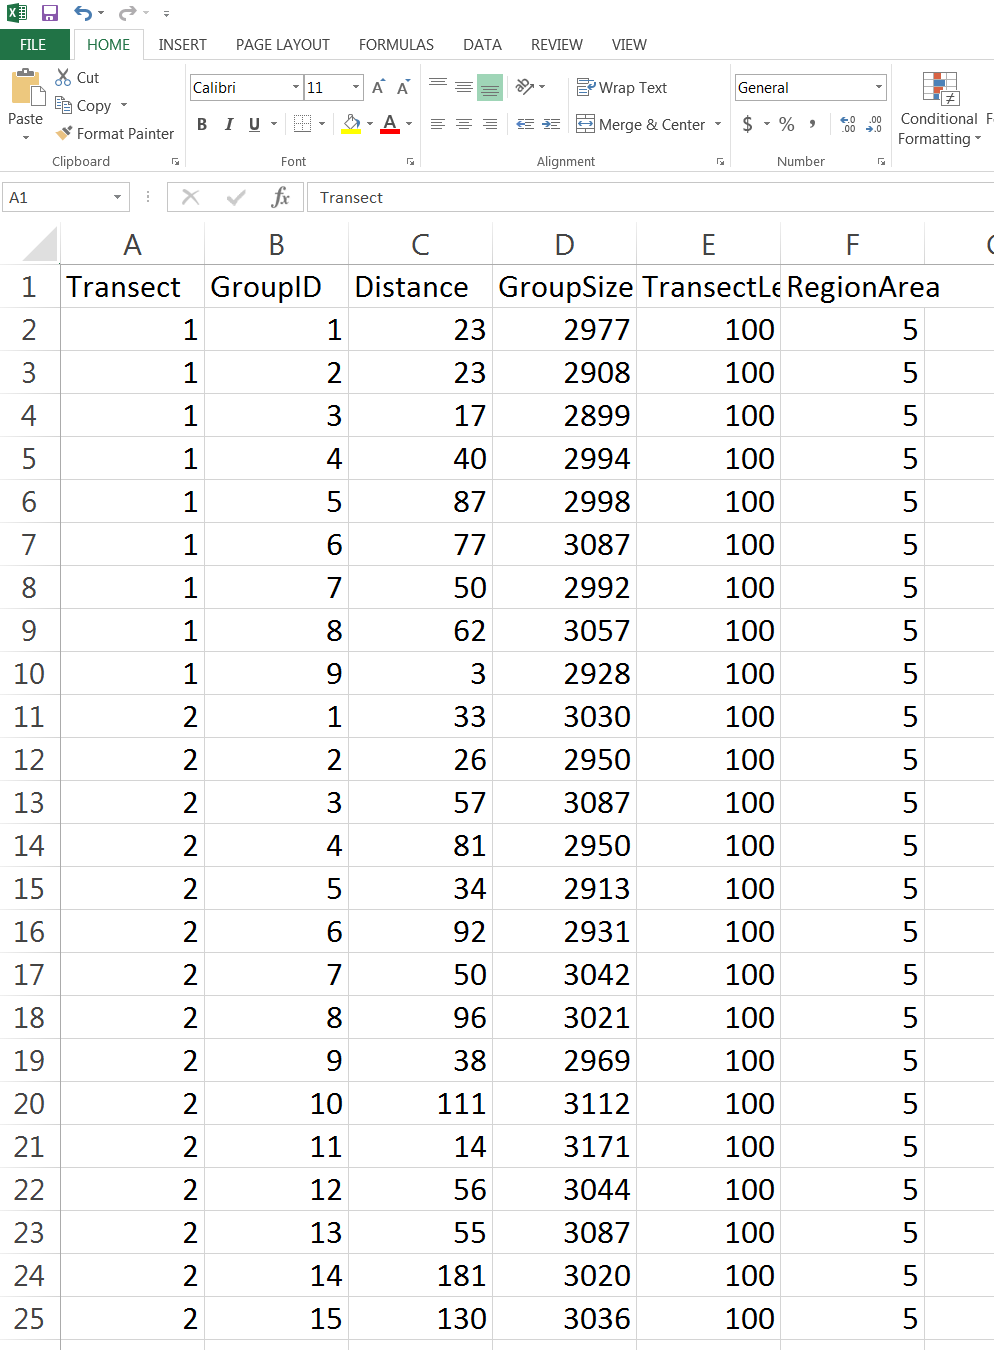
\includegraphics[height=8.5cm]{figs/ds-data1}} \hfill
%   \fbox{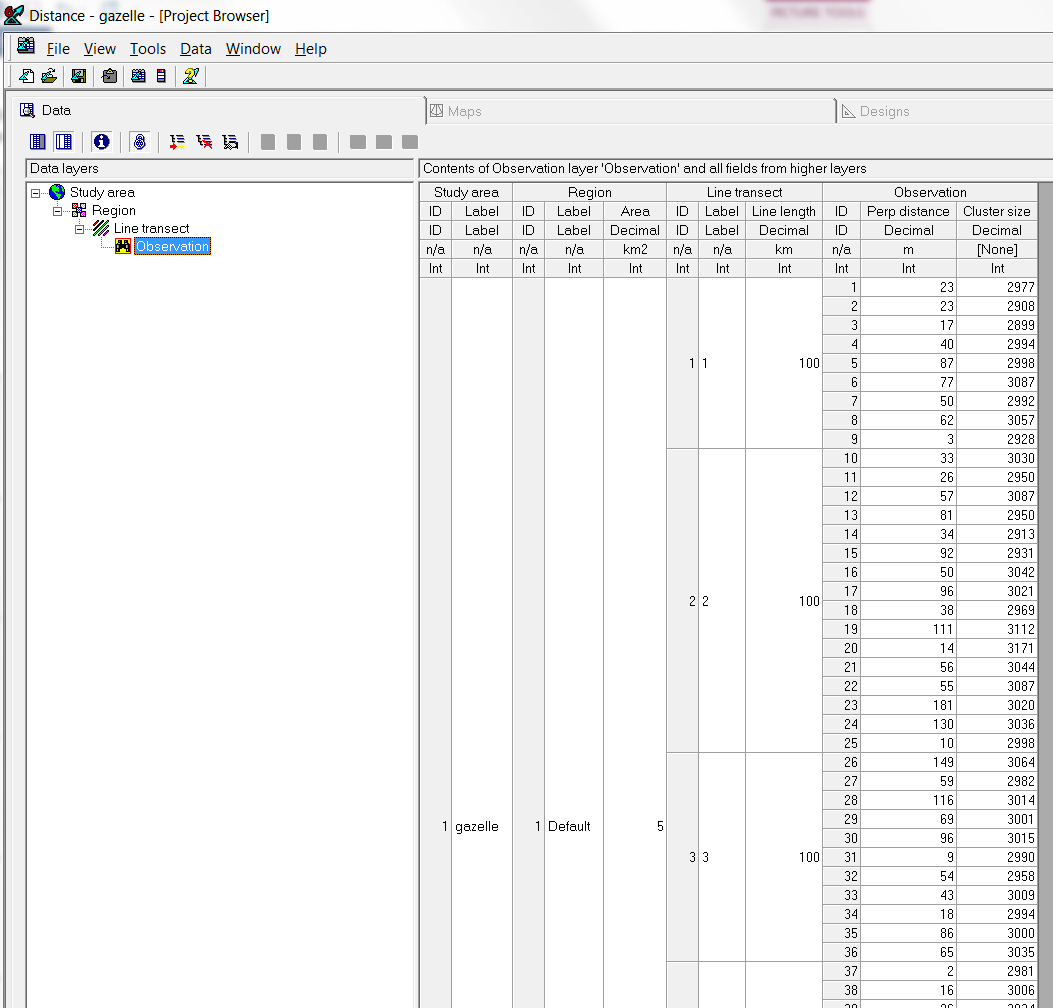
\includegraphics[height=8.5cm]{figs/ds-data2}}   \\
%   \caption{\small Data formatted in Excel (left) and the same data in
%     program DISTANCE.}
%   \label{fig:ds-data}
% \end{figure}
%\clearpage



%\clearpage

\section*{\large  Part II: Closed-population models in MARK}
The data file (\verb+CH-SO-Andy07.inp+) is a simple text file, formatted
as required by program MARK. Each row of the file is a capture history
for each of the 17 turtles captured in 2007 (May 31 - June 5). There
were 6 capture occasions, so for every turtle, there are 6 ones and
zeros indicating if the turtle was captured on that occasion or
not. After each capture history is a space followed by a 1 and a
semi-colon to indicate that there was just 1 turtle with this history.

\begin{figure}[h!]
  \centering
  \fbox{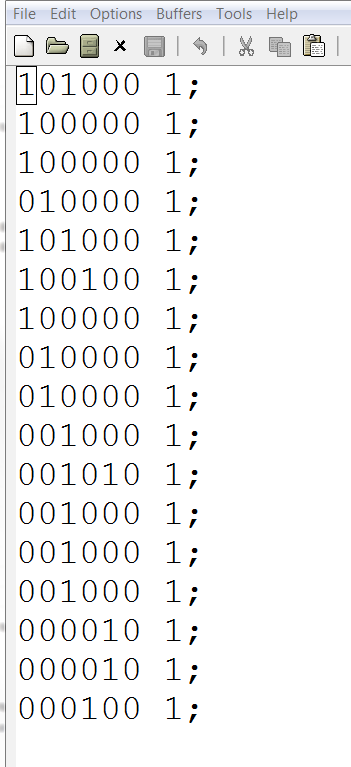
\includegraphics[height=7.5cm]{figs/stinkpot07-data}}
  \caption{\small Stinkpot capture histories in a text file ready to
    be imported to MARK.}
  \label{fig:stink07-data}
\end{figure}

\clearpage

{\bf Instructions}
\begin{enumerate}
  \item[(i)] Open MARK and create a new project by selecting:
    \verb+"File > New"+.
  \item[(ii)] Name the project ``Exercise I'' and select the capture
    history file \verb+``CH-SO-Andy07.inp''+ (see
    Fig.~\ref{fig:stink07-data})
  \item[(iii)] Choose \verb+"Closed Captures"+ from the list and select
    \verb+"Full likelihood p and c"+.
  \item[(iv)] Set the number of encounter occasions to 6, then hit
    \verb+"OK"+
\end{enumerate}

\begin{figure}[h!]
  \centering
  \fbox{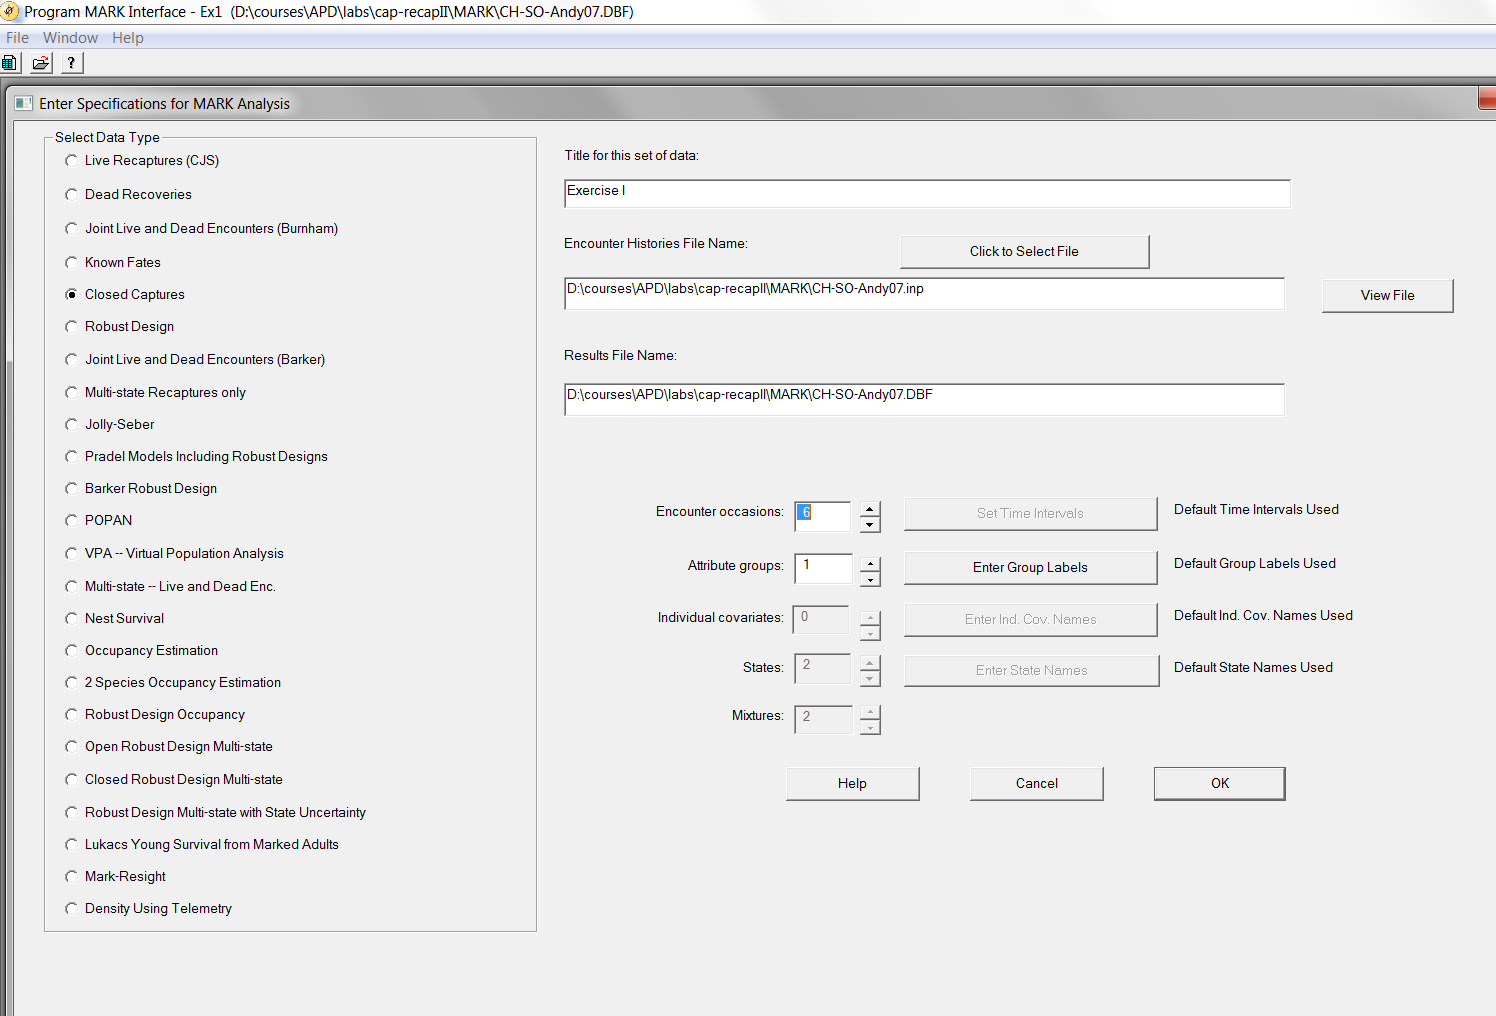
\includegraphics[width=0.9\textwidth]{figs/stinkpot07-MARK}}
  \caption{\small Setting up the MARK analysis of the stinkpot data.}
  \label{fig:stink07-mark}
\end{figure}

\begin{enumerate}
  \item[(v)] Run a model in which capture probability ($p$) and
    recapture probability ($c$) are constant by selecting
    \verb+"Run > Pre-defined Model(s)"+.
  \item[(vi)] Click the \verb+"Select Models"+ button and then choose the
    \verb+"(.)"+ option for $p$, $c$, and $N$. Click \verb+"OK"+, then
    hit \verb+"OK to Run"+.
  \item[(vii)] Right-click on the model name in the Results Browser
    and look at the \verb+"Real Estimates"+ to see the results.
  \item[(viii)]	Now, run two more pre-defined models: one with
    time-specific capture probabilities \verb+"p(t)"+ and one with
    time-specific recapture probabilities \verb+"c(t)"+. These two models can
    be run using the same steps above but by choosing \verb+"(t)"+ instead
    of \verb+"(.)"+.
\end{enumerate}

\clearpage

{\bf Assignment}

\begin{enumerate}
  \item[(a)] Summarize your results by creating a table in which each row
    is a model, and include the following columns: the estimates of $N$
    (abundance), the standard errors of $N$ (SE), and the AICc values.
  \item[(b)] The model with the lowest AICc is considered the best in
    the set of models. Which model has the lowest AICc? Do your
    results suggest that it is important to account for variation in
    capture (and recapture) probability over time? Explain.
  \item[(c)] What other sources of variation in capture probability do
    you think we might want to account for to obtain more reliable
    abundance estimates?
\end{enumerate}


\end{document}




